\documentclass[cic,tc,english]{iiufrgs}

% ----------------------------------------------------------------
% Initial Packages
% 
% Refs:
% https://github.com/schnorr/infufrgs/blob/master/exemplos/cic-tc.tex

% Use unicode
\usepackage[utf8]{inputenc}   % pacote para acentuação

% Necessário para incluir figuras
\usepackage{graphicx}         % pacote para importar figuras
\usepackage{svg}

\usepackage{times}            % pacote para usar fonte Adobe Times
% \usepackage{palatino}
% \usepackage{mathptmx}       % p/ usar fonte Adobe Times nas fórmulas

\usepackage[alf,abnt-emphasize=bf]{abntex2cite}	% pacote para usar citações abnt

% ----------------------------------------------------------------
% Other Custom Packages
% 

\usepackage{csquotes}
\usepackage{hyperref}
\usepackage{subcaption}
\usepackage{float}
\usepackage{blindtext}

% ----------------------------------------------------------------
% Code Listings
% 
% Provided by Alexandre Ilha (MSc Thesis)
% 
% Refs:
% https://en.wikibooks.org/wiki/LaTeX/Source_Code_Listings
% https://ctan.org/pkg/listings
% https://mirrors.ctan.org/macros/latex/contrib/listings/listings.pdf
\usepackage{listings}

\lstdefinelanguage{P4}[]{C++}{
    morekeywords={accept, action, actions, apply, bit, const, control, default, default_action, header, in, inout, key, out, packet_in, parser, select, size, start, state, struct, table, transition}
}

\lstdefinelanguage{Zeek}[]{C++}{
    morekeywords={addr, const, count, event, export, global, local, module, port, print, priority, redef, timeout, when},
    morecomment=[l]{\#}
}

\lstdefinelanguage{Bash}[]{}{
    morekeywords={},
    morecomment=[l]{\#},
    moredelim=[is][\bfseries]{<@}{@>}
}

\lstdefinelanguage{Py}[]{Python}{
    morecomment=[s]{"""}{"""},
    morekeywords={self}
}

\lstdefinestyle{code}{
    breaklines,
    basicstyle=\ttfamily\scriptsize,
    captionpos=t,
    floatplacement=htb,
    frame=tb,
    keywordstyle=\bfseries,
    numbers=left,
    numbersep=5pt,
    numberstyle=\ttfamily\tiny,
    showspaces=false,
    showstringspaces=false,
    tabsize=2
}

\lstdefinestyle{p4}{
    style=code,
    language=P4
}

\lstdefinestyle{zeek}{
    style=code,
    language=Zeek
}

\lstdefinestyle{bash}{
    style=code,
    language=Bash
}

\lstdefinestyle{python}{
    style=code,
    language=Py
}

\lstdefinestyle{cpp}{
    style=code,
    language=C++
}

\lstdefinestyle{inline}{
    breaklines,
    basicstyle=\ttfamily\normalsize
}

\lstset{style=code}

\newcommand{\code}[1]{\texttt{#1}}
% TODO figure out why this messes up line breaks.
% \renewcommand{\code}[1]{\lstinline[style=inline]{#1}}

% ----------------------------------------------------------------
% Custom name and simple definitions
%
% ----------------------------------------------------------------
% Definitions of names that haven't been decided yet:
% 

\newcommand{\TheSolutionName}[0]{ZPO}
\newcommand{\TheCodeGeneratorName}[0]{Zeek-P4 Offloader}

\newcommand{\Offloader}[0]{Offloader}
\newcommand{\Offloaders}[0]{Offloaders}

\newcommand{\ProtocolTemplate}[0]{Protocol Template}
\newcommand{\ProtocolTemplates}[0]{Protocol Templates}

\newcommand{\zeekconn}[0]{\textit{Connection}}

% ----------------------------------------------------------------
% Definitions to make sure some words are standard
% 

% ==============================================================================
% Title and Translated Title
% ==============================================================================

\title{A Framework and Automatic Code Generation Mechanism for Enabling Intrusion Detection Systems at Data-Plane Speeds}

\translatedtitle{Um Framework e Mecanismo de Geração Automática de Código para Permitir Sistemas de Detecção de Intrusão em Velocidades de Planos de Dados}


% ==============================================================================
% General Information
% ==============================================================================

\author{Sonntag Hagen}{Lucas}
\advisor[Prof.~Dr.]{Paschoal Gaspary}{Luciano}
\coadvisor[M.Sc.]{da Silveira Ilha}{Alexandre}
\date{July}{2022}
\location{Porto Alegre}{RS}


% ==============================================================================
% Keywords
% ==============================================================================

\keyword{Zeek}
\translatedkeyword{Zeek}

\keyword{P4}
\translatedkeyword{P4}

\keyword{Security}
\translatedkeyword{Segurança}

\keyword{Data planes}
\translatedkeyword{Plano de dados}

% TODO: add more keywords



% ==============================================================================
% Document
% ==============================================================================

\begin{document}

\maketitle

% Chapters

\chapter*{Acknowledgements}

Acknowledgements...

\chapter*{Agradecimentos}

Agradeço aos meus pais Rejane Sonntag Hagen e Roberto Hagen por me proporcionarem uma educação de qualidade e me apoiarem em todos os momentos. Ao meu irmão Bruno e minha namorada Giulia que fizeram parte dessa trajetória, incentivando-me a seguir em frente e a não desistir.

Ao meu orientador, Prof.~Dr.~Luciano Paschoal Gaspary, que me guiou nessa árdua tarefa chamada TCC, sempre com paciência e sabedoria, compartilhando um pouco de todo o seu conhecimento e sua experiência. Ao doutorando MSc.~Jonatas Adilson Marques e ao MSc.~Alexandre da Silveira Ilha por compartilharem seu tempo sanando as minhas dúvidas e guiarem-me em minha pesquisa.

Agradeço também à intituição UFRGS e seus professores, onde iniciei uma jornada profissional, conheci grandes amigos e construí meu currículo. Sou imensamente grato por todas as oportunidades recebidas. Faço aqui menção dos professores Raul e Taisy Weber, Lucas Schnorr e Gabriel Nazar os quais tiverem um participação especional nessa jornada acadêmica.

Além disso, gostaria de agradecer aos meus amigos e colegas de curso, os quais foram muito importantes em minha trajetória acadêmica. Meciono, em especial, meus colegas de intercâmbio Bernardo, Emily e Iron, os quais se tornaram uma família no ano de 2020, durante o auge da Pandemia da COVID-19. Ainda no intercâmbio, agredeço ao meu orientador Prof.~Dr.~Reinhard Gotzhein e ao doutorando MSc.~Paulo Aragão, que me acolheram e mentoraram a minha passagem pela Technische Universität Kaiserslautern. 

Ademais, gostaria de mencionar os meus chefes de estágios e outros colegas de trabalho, com os quais dividi momentos de apredizado e de lazer: Lauro Souza e Breno Araújo, do estágio que realizei no Google Brasil no ano de 2021-2022; Daniel Thiel, Hélio Fuques e Hernandi Krames do estágio na AEL Sistemas no ano de 2018-2020.

Por fim, agradeço aos demais professores, mentores, familiares e amigos, que direta e indiretamente participaram da minha jornada acadêmica, transmitindo aprendizados, compatilhando ideias e bons momentos, dividindo momentos de angústia e também de alegria.

\clearpage

% palavras-chave
% iniciar todas com letras minúsculas, exceto no caso de abreviaturas

% Keywords precisam estar definidos ANTES do \maketitle

\begin{abstract}
Abstract....
\end{abstract}

\begin{englishabstract}
{TITULO EM PORTUGUES}
{palavras chaves}

Abstract em Portugues...


\end{englishabstract}




\listoffigures
\listoftables
% lista de abreviaturas e siglas
% o parametro deve ser a abreviatura mais longa

\begin{listofabbrv}{FPGA}
    \item[API]  Application Programming Interface
    \item[ARP]  Address Resolution Protocol
    \item[ASIC] Application-Specific Integrated Circuit
    \item[AST]  Abstract Syntax Tree
    \item[BMv2] Behavioral Model Version 2
    \item[C2]   Command and Control
    \item[DDoS] Distributed Denial of Service
    \item[DDR]  Double data rate
    \item[DoS]  Denial of Service
    \item[DPD]  Dynamic Protocol Detection
    \item[DSL]  Domain-specific Language
    \item[EE]   Zeek Event Engine
    \item[FPGA] Field Programmable Gate Array
    \item[FTP]  File Transfer Protocol
    \item[ICMP] Internet Control Message Protocol
    \item[IDS]  Intrusion Detection System
    \item[IP]   Internet Protocol
    \item[IPv4] Internet Protocol Version 4
    \item[IPv6] Internet Protocol Version 6
    \item[MT/s] Megatransfers per Second
    \item[NIDS] Network Intrusion Detection System
    \item[NPU]  Network Processing Unit
    \item[NTP]  Network Time Protocol
    \item[NVMe] Nonvolatile Memory Express
    \item[PAF]  Packet Analysis Framework
    \item[PCAP] Packet Capture
    \item[PDP]  Programmable Data Plane
    \item[PDU]  Protocol Data Unit
    \item[PFD]  Programmable Forwarding Device
    \item[POF]  Protocol Oblivious Forwarding
    \item[PPS]  Packets Per Second
    \item[PSI]  Zeek Policy Script Interpreter
    \item[RAM]  Random Access Memory
    \item[RNA]  Reconfigurable Network Analytics
    \item[RQ]   Research Question
    \item[SDN]  Software Defined Network
    \item[SDN]  Software Defined Network
    \item[SSD]  Solid State Drive
    \item[TCP]  Transmission Control Protocol
    \item[TTL]  Time-To-Live
    \item[UDP]  User Datagram Protocol
    \item[UID]  Unique Identifier
    \item[VoIP] Voice over Internet Protocol
\end{listofabbrv}


% lista de símbolos
% \begin{listofsymbols}{$\alpha\beta\pi\omega$}
%       \item[$\sum{\frac{a}{b}}$] Somatório do produtório
%       \item[$\alpha\beta\pi\omega$] Fator de inconstância do resultado
% \end{listofsymbols}

\tableofcontents

     % 10+
\chapter{Introduction}
\label{cap:introduction}

Introduction...

\section{Motivation}

% \section{Threat Model}
% Not sure where this section goes... leaving it here so we don't forget.
    % 2
\chapter{Background}
\label{cap:background}

% Maybe use "Background and State of the Art"


\section{Zeek}
\label{sec:bg:zeek}


% TODO: don't forget to explain this from chapter 3:
% It consists of two high-level components: the RNA Host Engine, which executes in one of Zeek's worker nodes inside the IDS cluster;

Zeek is a.... \cite{AboutZeek}

Zeek started as Bro, which was proposed by Paxson \cite{Paxson1999}.

\subsection{Packet Capture}

\subsection{Event Engine}
\label{sec:bg:zeek_ee}

\subsection{Packet Analysis Framework}
\label{sec:bg:zeek_packet_analysis}

\subsection{Policy Script Analyzer}
\label{sec:bg:zeek_psi}

% Alexandre Ilha: TODO Explain in Ch. 2 that Zeek's PSI is an event-driven mechanism.


\subsection{Candidate Operations for Offloading}
\label{sec:bg:zeek_candidate_operations}

\section{Programmable Data Plane}
\label{sec:bg:pdp}

\subsection{P4}
\label{sec:bg:p4}
      % 5
\chapter{Reconfigurable Network Analytics}
\label{cap:rna}



In this chapter, we present an extended version of the Reconfigurable Network Analytics (RNA), an approach for offloading some of Zeek's operations discussed in Section \ref{sec:bg:zeek_candidate_operations} to programmable forwarding devices compatible with P4. This proposal is an extended version of the Reconfigurable Network Analytics (RNA) framework, which was initially proposed by  \citeonline{Ilha2022}. Since we advance on the original RNA, we describe the solution resulting from both, highlighting the new functionality.

\begin{figure}[h]
    \caption{RNA Framework}
    \begin{center}
        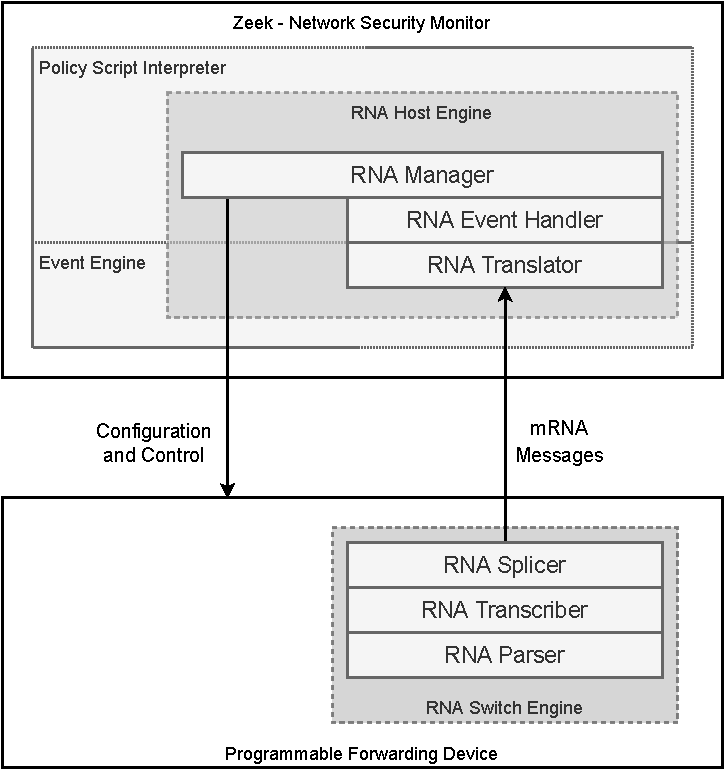
\includegraphics[width=0.7\textwidth]{images/arch_high_level.pdf}  
    \end{center}
    \label{fig:arch_high_level}
    \legend{Source: adapted from \citeonline{Ilha2022}}
\end{figure}

Figure \ref{fig:arch_high_level} illustrates the RNA framework. It consists of two high-level components: the RNA Host Engine, which executes in one of Zeek's worker nodes inside the IDS cluster; and the RNA Switch Engine, which is executed in a P4-programmable switch. Both components work together to offload packet analysis from Zeek to a programmable forwarding device. The RNA Switch Engine is able to parse packets and identify some of their characteristics, which are then summarized and sent to the RNA Host Engine. This summarized message is called mRNA. When the IDS receives this message, it is first processed by our Host Engine. It then converts the summarized message into Zeek's native structures, which can then be forwarded to Zeek's normal processing pipeline. This procedure allows us to bypass some operations that would be costly (such as protocol parsing and state tracking), and deliver this information closer or even directly to the Policy Script Interpreter (PSI, Section \ref{sec:bg:zeek_psi}), without disturbing Zeek's flow. By doing so, we make it so that no change is required on existing scripts running on the PSI.

% TODO: check what to call this "'custom software' to be executed both...."
In the original concept of RNA, depending on the IDS scripts chosen to be monitored by the operator, it is necessary to develop custom software to be executed both by the Host Engine and the Switch Engine. This ad-hoc development process quickly becomes impractical when we increase the number of desired scripts to be offloaded. For this reason, we propose an automatic code generation mechanism, described later in Chapter \ref{cap:code_gen}, which allows RNA to be a modular solution, where varying combinations of Zeek scripts can be chosen to be monitored, without the need to develop new software. Before detailing this automated process, we briefly review the operation of RNA components.

% ==============================================================================
%                               RNA OVERVIEW
% ==============================================================================
\section{RNA Components in a Nutshell}
\label{sec:rna:overview}

Using Figure \ref{fig:arch_high_level} as reference, we present the high-level components of the RNA framework and their functionality. We start with the RNA Host Engine, since it is the controlling part of the whole deployment, and then we describe the RNA Switch Engine.

% TODO: check if we'll remove the "RNA Event Handler" completely, or say it was removed but exists in the original RNA
The Host Engine unfolds into three components. The RNA Manager is the controlling component of the deployment, which first configures the P4 switch, setting up a monitoring session and loading all P4 code that is required to execute the offloaded tasks. After configuring the switch, it registers into Zeek all RNA Translators (one per-protocol of interest), so they receive mRNA messages. Translators are components responsible for waiting for such mRNA messages and translating them to Zeek native structures, and using those structures to trigger events, which are then consumed by the running scripts. The RNA Event Handler is another component that runs on the PSI and is initialized by the RNA Manager. It is designed as a debugging and logging component, capturing and handling events generated by the Translators.

The RNA Switch Engine is the program that executes in our P4-compatible programmable forwarding device. It has two components and we will be following the route of an incoming packet to explain them. The first component that processes a packet is the RNA Parser. It parses and extracts headers from each protocol, from the link layer, up to the application layer if required. After all the headers have been extracted, the packet enters P4's ingress pipeline, where the RNA Transcriber is executed. It extracts useful information from the packet and sets metadata that later will be used to build our summarized message, while also filtering some undesired packets. Having all the required metadata and going into P4's egress pipeline, the RNA Splicer builds and sends our summarized message, the mRNA, to the Host Engine with all information it may require to trigger a native Zeek Event.

Another important structure is the mRNA Message. It is a summary of a packet, summarizing all the information that the Switch Engine was able to extract from it. Sending an mRNA message is more efficient than sending a whole packet because the original packet contains headers that would still need to be parsed, information that, in some cases, is not necessary, and is not validated. In the summarized message, all information from L2 up to the L7 layer is gathered, filtered, and, in some cases, even formatted according to Zeek's native structures, saving Zeek from doing these operations on its own. The information-gathering process still needs to happen, but it is offloaded to the Switch Engine, which runs in a purpose-built device, making it much more efficient for this task. So the more information the switch is able to extract, the less Zeek has to do.

In an ideal world scenario, we would like to extract all information that Zeek needs to trigger an event, but sometimes that is not possible. Zeek's internal structures track connection states and use detection heuristics, which, because of P4's limited processing power for general tasks, we are unable to implement. This requires the mRNA message to be modular, allowing us to send, together with it, a part of the packet that was not able to be processed in the switch. This ensures P4 extracts all information it can, leaving the rest for Zeek to finish analyzing.

% ==============================================================================
%                               RNA DETAILED ARCHITECTURE
% 
%  This includes modifications made to allow code generation
% ==============================================================================
% TODO: Change the name of this section
\section{Detailed Framework Design}
\label{sec:rna:detailed_design}

This proposed version of the RNA framework, different from the original framework, goes further and specifies another level of modules that make the framework adaptable to variable situations with varying sets of monitoring scripts. Before explaining the inner details of the framework, we will introduce two concepts that are fundamental for its understanding and will serve later as inputs for our code generator tool. Those concepts are \Offloader{} and \ProtocolTemplate{}:

\begin{itemize}
    \item An \textit{\Offloader{}} is a set of files and settings that allows RNA to offload a new scripts and events. Like the idea of a module, it can be added and removed to the deployment, without needing to develop new software or change existing components.

    \item A \textit{\ProtocolTemplate{}} is a set of files and settings that allows RNA to parse a new protocol. An \Offloader{} requires a set of \ProtocolTemplates{} to be able to parse and offload the desired scripts.
\end{itemize}

\begin{figure}[H]
    \caption{RNA Framework - Detailed view}
    \begin{center}
        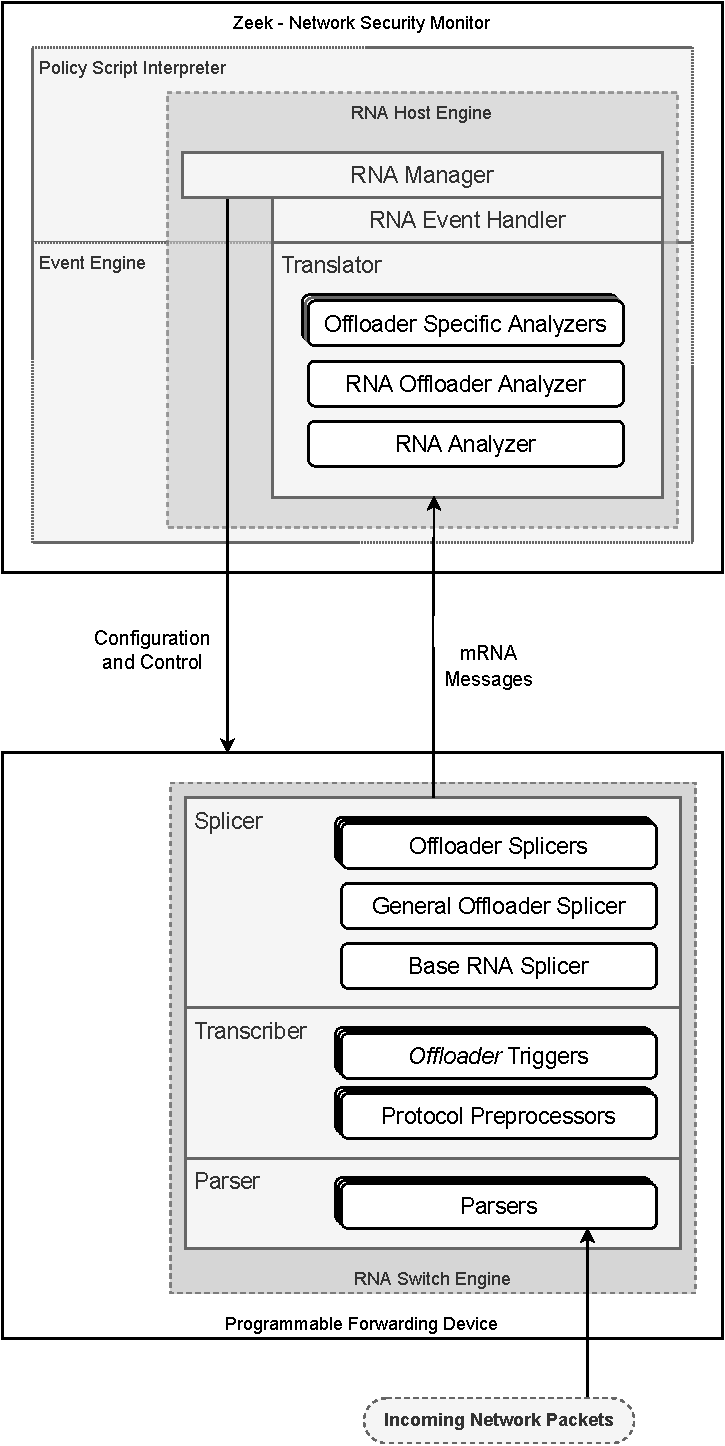
\includegraphics[width=0.6\textwidth]{images/arch_low_level.pdf}  
    \end{center}
    \label{fig:arch_low_level}
    \legend{Source: the author}
\end{figure}

In order to explain the details of the architecture behind RNA, presented in Figure \ref{fig:arch_low_level}, we use an example of an incoming ICMPv4 ping (\textsc{ICMP Echo Request}) packet and its trajectory through a deployed instance of RNA. In this fictional deployed system, the network operator also offloads other scripts that monitor protocols such as ARP, TCP, and UDP, which are not triggered by this specific incoming ping packet.

% Parei aqui.


\subsection{Switch Engine}

% Do we need this? Subsubsection directly after subsection.
\subsubsection*{The RNA Parser}

As the packet arrives at the P4-switch, it is first processed by the programmable parser. The RNA Parser component is a state machine with all the parsers the \Offloaders{} may need. Each one extracts its headers from the packet, and forwards the payload to the next parser. Each protocol's states and parsing instructions are provided by the \ProtocolTemplate{} of that specific protocol.

In our example which is shown in Figure \ref{fig:icmp_ex_parser}, the first parser would be the Ethernet parser, extracting its header, followed by the IPv4 and ICMP parsers. In the same figure, we also display other states of parsers that were not triggered, such as ARP, TCP, and UDP, each one provided by its own template. These unused protocol parsers are displayed by dotted lines, exemplifying where they would be linked in the general parser. After the packet's headers are parsed, it is sent to the ingress pipeline, where the RNA Transcriber will process the incoming data.

\begin{figure}[ht]
    \caption{Parsing States - ICMP Parsing Example}
    \begin{center}
        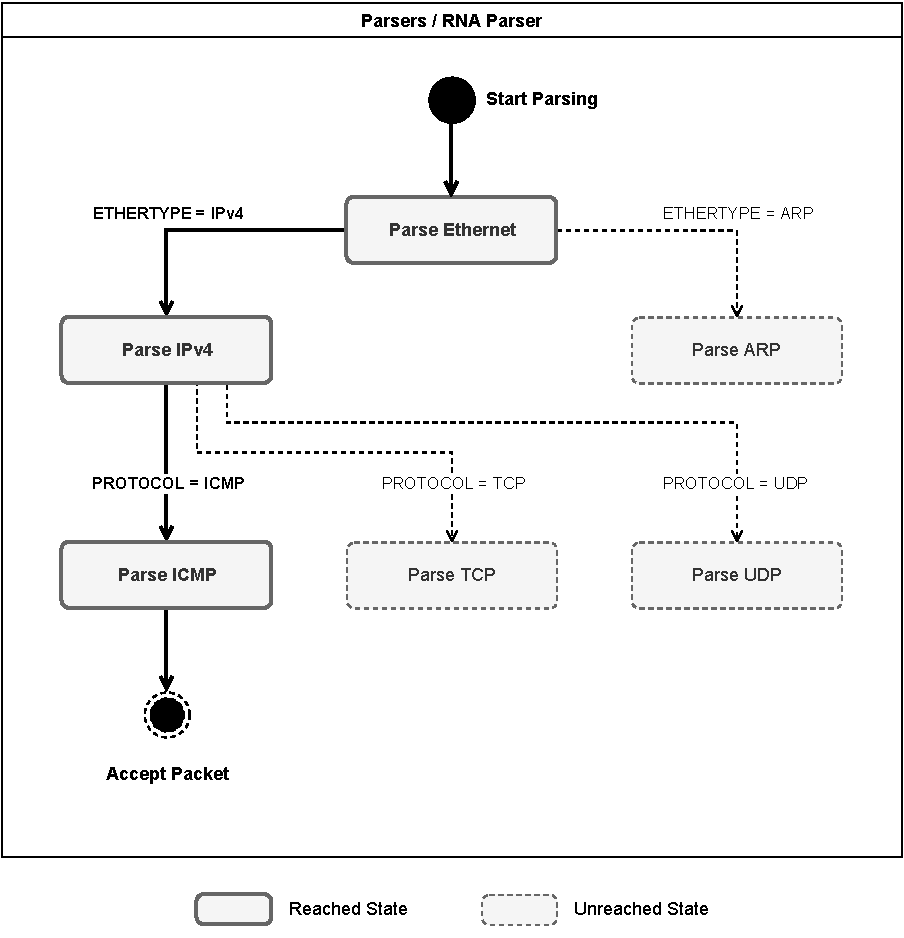
\includegraphics[width=0.7\textwidth]{images/icmp_ex_parser.pdf}  
    \end{center}
    \label{fig:icmp_ex_parser}
    \legend{Source: the author}
\end{figure}

\subsubsection*{RNA Transcriber}

In the RNA Transcriber, as shown in Figure \ref{fig:arch_low_level}, there are two types of modules, the Protocol Preprocessors, and the Offloader Triggers, both of which may have multiple instances. We start explaining the Protocol Preprocessors since they are the first modules to be executed inside this component.

The Protocol Preprocessors are functions that every \ProtocolTemplate{} may execute to extract protocol-related information from the packet, and save it to the metadata. This module is optional and every \ProtocolTemplate{} may have only one preprocessor. In our example, the processor extracts the ICMP type from the header and saves it in the metadata.

The next modules to be executed in the Transcriber are the Offloader Triggers, which are conditions that identify which \Offloader{} should be triggered. Each of these conditions is checked, and the first \Offloader{} to have its trigger condition valid is marked as the triggered one in the packet's metadata. In our example of an ICMP echo request, our trigger condition is \texttt{icmp.type = 8}. This ensures the \Offloader{} \textsc{ICMP Echo Request} is triggered when a ping packet has arrived.

% TODO: Maybe add here a code snippet

After a valid \Offloader{} is found, a copy of this packet is created, and using this cloned packet, the switch will be able to construct the mRNA message. The original packet will follow its flow and be delivered to the originally intended destination.

\subsubsection*{RNA Splicer}

The RNA Splicer is executed after the packet leaves the ingress pipeline and it enters the egress pipeline\footnotemark{}. The RNA Splicer is composed of three different types of Splicers, the RNA Base Splicer, the General Offloader Splicer, and the Offloader Splicers.

The RNA Base Splicer constructs the base header for the mRNA message. This is a simple header that contains the RNA version and the RNA message type. We decided to use this simple header to allow for more expandability in the future, for example, adding debugging and other types of messages.

% TODO: add code snippet of the header?

The next splicer, The General Offloader Splicer, constructs a header that contains general information, which all \Offloaders{} share, and is executed for every \Offloader{}. This information includes, for example, source IP, destination IP, L3, and L4 protocols, and triggered \Offloader{}. In our example of the ICMP ping request, the General Offloader Splicer sets both source and destination IPs, the L3 protocol to \texttt{IPv4}, the L4 protocol to \texttt{ICMP}, and the offloader type to \textsc{ICMP Echo Request}.

The third type of splicer is the Offloader Splicers. These are splicers that every \Offloader{} has. Each \Offloader{} Splicer constructs the header with the extra information required to execute its functionality, that was not yet present in the General Offloader Splicer. In our example, the \textsc{ICMP Echo Request} Splicer will construct a header with information about the ICMP ping packet: \texttt{type}, \texttt{code}, \texttt{sequence}, and \texttt{id}.

% TODO: Maybe add code snippets here too


\footnotetext{Since we are explaining the architecture behind RNA, we are not considering the inner workings of the programmable data plane, where a buffer connects the ingress and egress pipeline.}

After every Splicer has finished constructing its headers, the mRNA message will be ready. The payload and headers, which together form the mRNA, are then merged and sent to Zeek's monitoring interface, effectively finishing the processing on the Switch Engine. From now on, Zeek's Translators will work to support the monitoring infrastructure.

\subsection{Host Engine}

In this section, we describe how the Host Engine receives the mRNA messages and uses them to execute the monitoring scripts. Figure \ref{fig:arch_low_level} shows the first components of the RNA Framework to receive the mRNA message are the Translators. Before any RNA Analyzer (Translator) receives its packet, the packet is first received by Zeek's Ethernet Analyzer. When analyzing the packet, the previously registered mRNA ethertype code will ensure all mRNA messages are forwarded to our RNA Analyzer as shown in Figure \ref{fig:icmp_ex_translator}.

\subsubsection*{RNA Translator}

The RNA Translator, similar to the RNA Splicer, is composed of three different types of Analyzers, which are components responsible for parsing each layer of the mRNA message. We use Figure \ref{fig:icmp_ex_translator} to explain how the analyzers connect to each other. First, it is important to note that Analyzers with a gray background are Zeek provided, and Analyzers with a dashed border are Analyzers present in our deployment, but they are not executed due to our ICMP ping packet example (explained at the beginning of Section \ref{sec:rna:detailed_design}).

\begin{figure}[ht]
    \caption{Analyzers - ICMP Translation Example}
    \begin{center}
        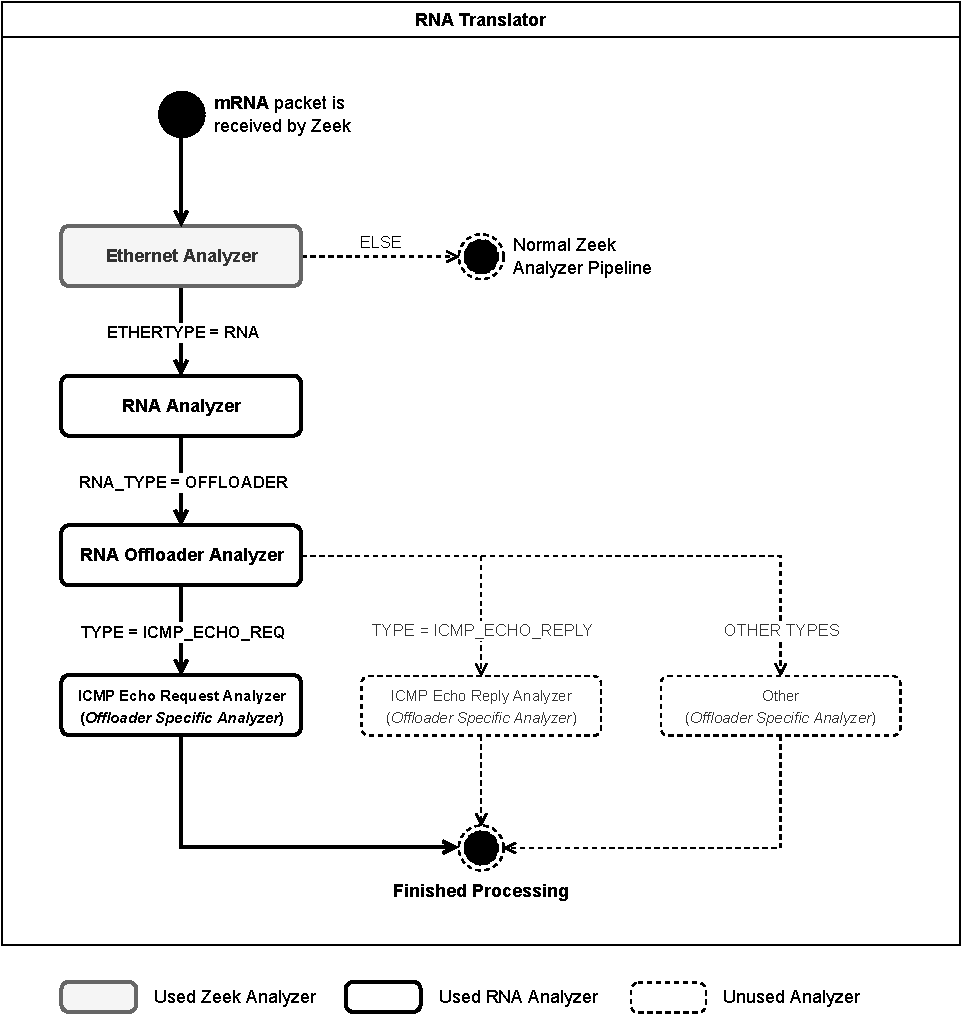
\includegraphics[width=0.8\textwidth]{images/icmp_ex_translator.pdf}  
    \end{center}
    \label{fig:icmp_ex_translator}
    \legend{Source: the author}
\end{figure}

The RNA Analyzer is the first Analyzer of the RNA architecture to receive the mRNA packet. As explained in the previous section, the RNA protocol has a generic header that indicates only the protocol version and the message type. This is the header that is extracted by the first Analyzer. In the case of this project, the only message type we use is the \Offloader{} type\footnotemark. Using our previously described example of the ICMP ping, the mRNA packet created for the ICMP ping will have its type as \textsc{\Offloader{}}, forwarding it to the RNA Offloader Analyzer.

\footnotetext{There are actually three types of \Offloaders{}, but for simplification purposes, in this description we present the Offloader type as being one unique type.}

Next, the RNA Offloader Analyzer is the second Analyzer of our RNA implementation to receive the mRNA packet. It parses the header generated by the General Offloader Splicer with \Offloader{} generic information. This Analyzer is also responsible for forwarding the mRNA packet and its payload to the \Offloader{} specific Analyzer by using the \Offloader{} \texttt{type} code. In our example, the next Analyzer to be executed is the \textsc{ICMP Echo Request} Analyzer. It is also important to note we display in Figure \ref{fig:icmp_ex_translator} two other Analyzers, displayed with dashed borders, that are present in the deployment but were not triggered due to the \Offloader{} type of this specific example packet: \textsc{ICMP Echo Request}.

The last Analyzer to be executed is the Offloader Analyzer. This is a module every \Offloader{} must have. It is responsible for converting the received information to Zeek's native structures. It can then trigger one or more desired events, which will be consumed by the monitoring scripts. In our example, the \textsc{ICMP Echo Request Analyzer} is going to trigger Zeek's native \texttt{icmp\_echo\_request} event. By triggering this event, we ensure all scripts that use it will perform exactly as Zeek had processed the ICMP ping request entirely in its own infrastructure.

As explained previously, an Analyzer directly triggering a Zeek Event is the ideal case, but not always possible. In the cases this is not possible, the Analyzer has the option to extract the mRNA headers and forward the rest of the payload to another Zeek-provided Analyzer. This other Analyzer, which is already part of Zeek's infrastructure, can then analyze the packet and trigger the proper events.
             % 10 (or 20 if no implementation chapter)
\chapter{Automatic Code Generation for RNA}
\label{cap:code_gen}

In this chapter, we present a mechanism for automatic code generation for the RNA Framework. This enables network operators to deploy the framework without having the experience and knowledge to develop software for Zeek or programmable forwarding devices (P4).

The code generation mechanism uses two sets of inputs: the Zeek scripts, whose events should be offloaded, and a pool of Protocol Templates and Offloader Templates (whose concepts we introduced in \autoref{sec:rna:detailed_design}). These constructs are used as sources of templates and resources in order to implement the software required to offload the events subscribed by the desired scripts. We also propose the generation of a single Zeek Plugin package, which, when initiated, automatically deploys the code for both the Host Engine and the Switch Engine (instead of having two separate deployable packages).

% ==============================================================================
%                               OVERVIEW
% ==============================================================================

\section{Overview}
\label{sec:code_gen:overview}

In this section, we present an overview of the RNA Code Generation Mechanism, starting with its inputs and expected output, which is illustrated in \autoref{fig:code_gen_black_box}. The main input for the mechanism is the set of Zeek scripts, whose monitoring the network operator is interested in. These scripts need to be provided in their entirety, so we can identify the events to which they subscribe.

\begin{figure}[htb]
    \caption{RNA - Code Generation Mechanism}
    \begin{center}
        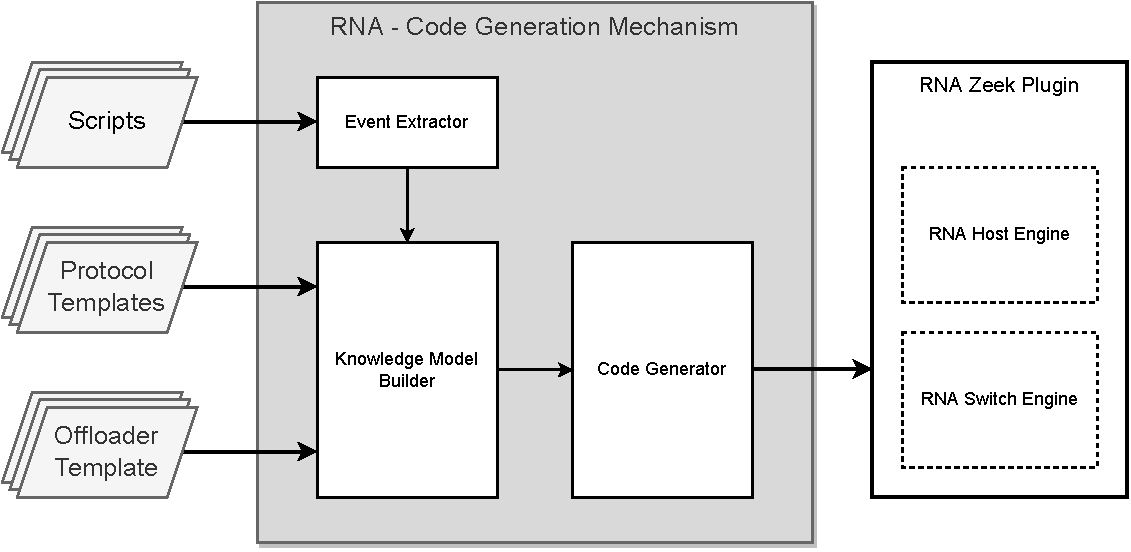
\includegraphics[width=0.98\textwidth]{images/code_gen_mechanism.pdf}
    \end{center}
    \label{fig:code_gen_black_box}
    \legend{Source: the author (2022).}
\end{figure}

The second set of inputs is what we call \textit{templates}, which can be either  Protocol Templates or Offloader Templates. They are a pool of known implementations of protocols and events that can be used to offload scripts. A template being present in this pool does not mean it will be included in the final output, but it means it is available in case its implementation is needed by a script.

The desired output of our mechanism is a single Zeek Plugin following the structure previously presented in \autoref{sec:rna:overview} and illustrated in \autoref{fig:arch_low_level}. This Zeek Plugin, when executed, should: configure the switch by creating a mirroring session for the Zeek monitoring system and deploying the P4 code; and configure Zeek by registering all Translators in Zeek's Event Engine and loading the RNA Event Handler. This eliminates the need for the operator to coordinate the deployment of two separate systems, i.e., the RNA Host Engine and the RNA Switch Engine.

To be able to execute this task, the first objective of the code generation process is to analyze all the provided Zeek scripts and identify which are the observed events in every script. Once this pool of events is known, we select Offloaders (from the templates pool) that are capable of offloading those events. This step is finished and succeeds if we find at least one Offloader for every event.

After all events and Offloaders have been selected, the mechanism must ensure all templates for the protocols required by these Offloaders are available. The Protocol Templates are required so the Offloaders can interpret the desired headers. After all this knowledge model is complete, the mechanism generates all required source files.

Some of the resulting code that is present in the final Zeek Plugin is extracted and merged from the templates and is not entirely generated by our mechanism. It is not yet possible to fully generate all offloader code because the process of converting C++ or P4 code from one to another is very complicated and is out of the scope of this project.


% ==============================================================================
%                            Detailed Mechanism Design
% ==============================================================================

\section{Detailed Mechanism Design}
\label{sec:code_gen:detailed}

The operation of our RNA Code Generation Mechanism can be described in three different stages. The first stage identifies the events that our input scripts subscribe to. The second stage is building our knowledge model, which receives as inputs all Protocol Templates, Offloaders, and events of interest, that the network operator requested to be offloaded. We call this knowledge model \textit{ProtocolGraph}. The last stage is the actual code merge and generation process using this structured and validated knowledge model from the previous step. We start explaining the first stage of our mechanism, i.e., extracting the subscribed events from the Zeek Scripts.

\subsection{Event Extraction}

To identify which events a Zeek Script subscribes to, we first need to parse the script as a whole. The mechanism does it using Zeek's provided grammatical definition. After parsing all the scripts, we search the Abstract Syntax Tree for event handlers, returning their event identifiers. \autoref{fig:event_extraction_example} illustrates a fragment of a Zeek Script that detects FTP Bruteforce attacks. For this particular example, the mechanism would identify the event handler declaration on line $20$, which is the \texttt{ftp\_reply} event.

\begin{figure}[htb]
    \caption{Section of a Zeek Script}
    \begin{center}
        \lstinputlisting[style=zeek]{code/example_zeek_script.zeek.txt}
    \end{center}
    \label{fig:event_extraction_example}
    \legend{Source: the author (2022).}
\end{figure}

In this stage, the most important information to be forwarded to the next step is the identifiers of the events we want to offload. Those will indicate the requirements of our deployment. The name of the scripts are also passed to the knowledge model as a logging and debugging asset but are no longer essential for the final functionality.

\subsection{Knowledge Model Builder}

The core logic behind the implementation of our RNA Code Generation Mechanism relies on a structure we call \textit{ProtocolGraph}. This is a graph structure that stores all protocols required for our events of interest. The Offloaders are linked to their final protocol layer in the graph, generating, in the end, a structure as presented in \autoref{fig:protocol_graph}. This structure is a graph, with a node we assign as root, in most cases, the \textsc{Ethernet} protocol. The other protocols are linked to their respective parents. The Offloaders are linked to the protocol they analyze, which does not need to be a leaf protocol.

\begin{figure}[htb]
    \caption{Knowledge Model - Protocol Graph}
    \begin{center}
        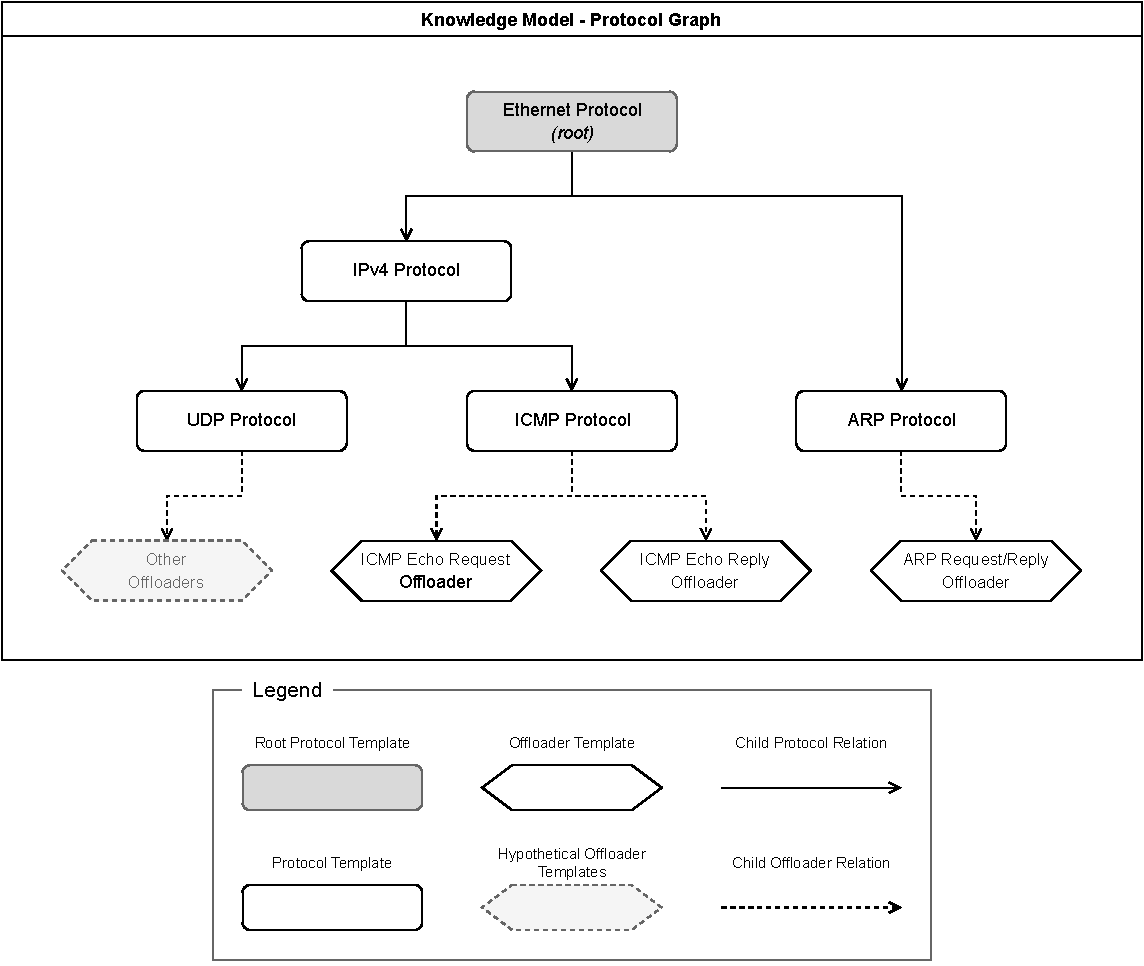
\includegraphics[width=0.98\textwidth]{images/icmp_ex_protocol_graph.pdf}  
    \end{center}
    \label{fig:protocol_graph}
    \legend{Source: the author (2022).}
\end{figure}

The procedure to generate and validate the \textit{ProtocolGraph} is outlined in \autoref{alg:build_graph}. The pseudo-code will be used to describe and guide the explanation of our method, and we will refer to the lines according to their respective roles.

\begin{algorithm}[htb]
    \caption{Knowledge Model Build Algorithm}
    \label{alg:build_graph}
    \SetKwInput{Input}{Input}
    \SetKwInput{Output}{Output}
    
    \Input{$templates$, $events$, $forced\_of\!floaders$}
    \Output{$graph$}
    
    \vspace{1em}

    \Call{ValidateComponentList}{$templates$}

    \vspace{1em}

    $protocols \gets$ FilterListByType($templates$, $ProtocolTemplate$) \\
    $of\!floaders \gets$ \Call{FilterListByType}{$templates$, $Of\!floaderTemplate$} \\
    
    \vspace{1em}
    
    $of\!floaders \gets$ \Call{ReqOffloaders}{$of\!floaders$, $events$, $forced\_of\!floaders$} \\

    \vspace{1em}

    \If{$of\!floaders$ is empty} {
        \textbf{raise} \textit{exception} \Comment{nothing to be offloaded}\\
    }

    \vspace{1em}

    $root \gets$ \Call{FindRootProtocol}{$protocols$} \\
    $graph \gets$ \Call{LinkGraph}{$root$, $protocols$} \\

    \vspace{1em}

    \If{\Call{HasCycles}{$graph$}} {
        \textbf{raise} \textit{exception} \Comment{protocol graph has cycles}\\
    }
    
    \vspace{1em}
    
    $protocols \gets$ \Call{RemoveUnreachableProtocols}{$graph$, $protocols$} \\
    \Call{AttachOffloaders}{$graph, of\!floaders$} \\
    
    \vspace{1em}

    \Call{TrimUnusedProtocols}{$graph$} \\
    
    \vspace{1em}
            
    \Call{SetProtocolDepths}{$graph$} \\
    \Call{SortProtocols}{$graph$} \\
    \Call{SortOffloaders}{$graph$} \\
    \Call{SetOffloadersUids}{$graph$} \\
    
    \vspace{1em}
            
    \textbf{return} $graph$ \Comment{successful graph generation} \\
    % \legend{Source: the author (2022).}
\end{algorithm}


\subsubsection*{Template loading and filtering}
% Lines 1 - 6

As the mechanism is executed, the first step is to load all templates and validate their versions, files, and requirements. All the templates are loaded and stored in a list, even if they are not used later in the final model. After they are loaded, we separate them between Protocol Templates and Offloader Templates (\autoref{alg:build_graph}, lines 1-3).

After all offloader templates are validated, we select what offloaders are required (line 4). This selection process is based on two parameters: the event identifiers (provided by the Event Extraction stage) and a list of ``forced'' offloaders (provided by the network operator when invoking the code generator mechanism). The first offloaders to be assigned as required are the ones explicitly requested by the network operator. Next, we select an offloader for each event, ensuring all events are covered. If, at the end of this process, one or more events do not have offloaders associated with them, the process fails and is aborted. Otherwise, we proceed. We then check if the list of Offloaders is not empty and proceed to the next section (lines 5-6).

\subsubsection*{Graph building}
% Lines 7 - 13

After the templates have been validated and the desired Offloaders have been selected, the mechanism needs to find the root protocol. If none or more than one root Protocol Template is found, an exception is raised, and the process is terminated (line 7).

Each Protocol Template has its own identifier, which is a unique string, as well as the identifiers of the parent protocols. Using these identifiers, the Protocol Templates are linked to their parent, making sure the links are all valid (line 8), for example, the ICMP protocol is linked to its parent protocol, the IPv4. After linking, the algorithm validates there are no cycles on the protocol graph (lines 9-10). The reason the protocol graph can not have cycles is due to limitations on the algorithm's P4 implementation, where protocol headers can not be parsed twice for a single packet. By ensuring no cycles are present in the \textit{ProtocolGraph}, we ensure protocol headers can only be used once. After the graph is built, the algorithm removes all unused protocols from the protocol list (line 11).

The algorithm links all the required Offloaders to their respective protocols (line 12). If any Offloader fails to be attached to its protocol, the algorithm aborts the execution. At this point, the \textit{ProtocolGraph} is fully built, but it may have unnecessary protocols still attached to it. These protocols that have no Offloaders attached to them or any Offloaders attached to their child protocols are removed on line 13. It might sound strange that we build the graph to then trim and optimize it. Since the development of this mechanism was incremental, this is how it was originally developed, but we acknowledge it could be further optimized.

We acknowledge that this implementation is not the optimal implementation and that it could be further optimized.

\subsubsection*{Sorting and Prioritization}
% Lines 14 - 17

After the \textit{ProtocolGraph} is fully built, the mechanism sets the last metadata that will be needed in the code generation stage. The first metadata to be set is the \textit{protocol depth}. For each protocol, the mechanism sets protocol depth as the maximum distance of that protocol to the root protocol (line 14). The depth is used to then sort the protocols and their Offloaders in a list (lines 15 and 16), which will later be consumed by the code generator. A list based on Offloader priority is also created at this time. The last step is to set the unique identifier (UID) for the Offloaders (line 17). This ensures the Switch Engine and the Host Engine have the same identifier referring to the same Offloaders.

\subsection{Code Generation}

The code generation is based on a \textit{master template} with blank slots, which are filled with the generated code. The code that fills the slots of the master template is either fully generated by the mechanism or is pulled from the protocol and Offloader templates.

Next, we first describe how the code is generated for the P4 switch, and then we explain how it is generated for the Zeek Plugin. This code generation process could be, in most parts, parallelized since it is based on the previously generated \textit{ProtocolGraph}, but we did not see the necessity to implement the parallelism at this time.

\subsubsection*{Code Generation for the Programmable Switch (P4)}

The P4 code is mainly composed of three files, which are \textit{headers.p4}, \textit{parser.p4}, and \textit{main.p4}. We explain this structure in a bottom-up approach, starting with the headers file. The headers file, as the name suggests, contains all the headers and data structures required by the output program. It is generated by merging all headers provided by the templates, which include protocol headers, mRNA headers, and Offloader specific headers\footnotemark{}, and others. 

% In this file, the mechanism also generates \textcolor{blue}{the structure that holds all headers, this is where parsed protocol headers will be saved for each packet}. This structure is generated using the previously-sorted lists of protocols and offloaders because the protocols need to be inserted into the structure according to their layering order. The first header to be included is the root protocol, followed by the rest of the protocols (starting with lower-layer protocols), then the mRNA headers, and finally the Offloader-specific headers, which are the last ones to be added.

\footnotetext{The Offloader specific headers are headers created by the Offloader Splicer, which were explained in \autoref{sec:rna:detailed_design}.}

The \textit{parser.p4} file contains all the information required for parsing and deparsing protocols. The parser, as described previously in \autoref{sec:rna:detailed_design}, is a state machine. The states of the parser are all generated based on the information provided by the protocol templates. It uses the next protocol selector field to select one of the child protocols. Using our example from \autoref{sec:rna:detailed_design}, shown in \autoref{fig:icmp_ex_parser}, the Ethernet parsing state would use the \texttt{ethernet.ethertype} field to select either the \textit{IPv4} or \textit{ARP} protocols. When parsing our example \textsc{ICMP Echo Request} packet, the value of the ethertype field would point to IPv4. Likewise, the value of the \texttt{Protocol} field in the IPv4 datagram would point to ICMP.

To support protocols with variable-size headers, the template has the option to use a custom parsing code, which replaces the default header extractor. Instead of extracting a fixed-size header based on a (fixed-size) structure, this custom code allows the templates to determine the received header size and parse the right amount of bits from the packet.

% For deparsing and sending an mRNA message, the mechanism does not need to generate any complex code. Since all our headers have already been sorted in our header holding structure (defined in the \textit{headers.p4} file), all the mechanism needs to do is to generate an \textit{emit} command with all headers of a packet. When this code is executed, the P4 switch will check and emit only valid protocols, eliminating the need for us to generate a code section checking the validity of each protocol.

The main P4 file is the entry point for our P4 program. It defines the ingress and egress pipeline control structures while also loading the headers and the parser files. When generating the ingress pipeline, we split it into two generated sections, the \textit{protocol preprocessors}, and the \textit{Offloader triggers}. The protocol preprocessors section is generated by merging the preprocessors provided by every protocol template, which were explained in \autoref{sec:rna:detailed_design}. The preprocessors are each wrapped with verification to ensure the protocol is valid for that packet, and are generated in bottom-up order. \autoref{fig:ingress_pipeline_ex} shows an example of a section of the ingress pipeline. The generated protocol preprocessors are displayed on lines 3 - 16, where each of the preprocessors is wrapped with an \textit{if statement} to ensure the protocol is valid before executing the preprocessor.

Still in the ingress pipeline, the Offloader triggers are conditions provided with every Offloader template and are also wrapped with a test for protocol validity. They are sorted based on the Offloader's priority since only one Offloader may be triggered per packet. This is an if statement, which, when met, sets the \texttt{metadata.offloader} field to the Offloader's UID, which is defined in the \textit{ProtocolGraph}. Using \autoref{fig:ingress_pipeline_ex} again as an example, on lines 20 - 39 the Offloader triggers are defined. The trigger condition for the \textit{NTP Message Offloader} is seen on line 26. If this condition is true, the P4 switch will set the \texttt{meta.offloader\_type} field to \texttt{RNA\_NTP\_MESSAGE\_UID} (line 27).


\begin{figure}[htb]
    \caption{Section of the P4 Ingress Pipeline}
    \begin{center}
        \lstinputlisting[style=p4]{code/ingress_pipeline.p4.txt}
    \end{center}
    \label{fig:ingress_pipeline_ex}
    \legend{Source: the author (2022).}
\end{figure}

Still in the \textit{main.p4} file, the egress pipeline is composed of one generated section, the \textit{Offloader splicers}. This code section is composed of \textit{if} statements verifying the metadata's Offloader identifier. In the \textit{if} body, the mechanism merges the splicer code, which is provided by every Offloader template and will be executed if the Offloader UID matches the one in the metadata. \autoref{fig:egress_pipeline_ex} shows an example of the splicer section of the egress pipeline. Lines 2 and 6 verify the triggered offloader, and lines 3 - 5 and 7 - 9 are the splicer code for the \textit{FTP Message Offloader} and the \textit{NTP Message Offloader}, respectively.

\begin{figure}[htb]
    \caption{Section of the P4 Egress Pipeline}
    \begin{center}
        \lstinputlisting[style=p4]{code/egress_pipeline.p4.txt}
    \end{center}
    \label{fig:egress_pipeline_ex}
    \legend{Source: the author (2022).}
\end{figure}

\subsubsection*{Code Generation for the Zeek Plugin package}

The generation of the Zeek Plugin is much simpler than the P4 code generation. Most of the Zeek Plugin is composed of static files, which are copied from the \textit{master template} and from the templates. The rest of the generation consists of registering the template's Analyzers, defining constants, and creating \textit{read me} and \textit{version} files.

The most important files to be generated are the main plugin file (\texttt{Plugin.cc}), the main Zeek Script file (\texttt{main.zeek}), and the building rules (\texttt{CMakeLists.txt}). The main plugin file needs to include the C++ header files and register the Analyzers. The main Zeek Script file needs to contain instructions to load the Analyzers and bind them to the specific Offloader UIDs, which were defined by the \textit{ProtocolGraph}. To ensure all the template's code files are properly compiled, the mechanism needs to add all their file paths to the \textit{CmakeLists} recipe. The last step in the composition of the Zeek Plugin package is to generate the \texttt{README} file, which describes what the plugin does, and the \texttt{VERSION} file, which contains the version of the generated plugin.

The proposed mechanism was conceived to embed the P4 code in the Zeek Plugin package so that when the RNA Manager is initiated, the P4 code can be deployed to the programmable forwarding device. This was not implemented in the prototype, but we briefly describe how it could be implemented. This could be implemented by first generating the P4 code, then compiling it, either with a P4 command or even in a Docker container, to ensure all dependencies are met. After that, when generating the Zeek Plugin package, the mechanism would embed the output of the P4 code compilation (a \textit{JSON} file) and generate a function to load it to the switch when the RNA Manager was initialized.

        % 10
\chapter{Proof of Concept and Evaluation}
\label{cap:evaluation}

In this chapter, we present how the automatic code generation mechanism proposed in \autoref{cap:code_gen} was implemented in a fully functional proof of concept. We also describe how we evaluated the gains in performance and ease of development and deployment for users of our framework.

To facilitate the development of this project and to keep the scope within a defined limit, we did not use P4-compatible hardware. Instead, we used the Behavioral Model version 2 (BMv2) software-based switch \cite{BMv2} to run the P4 code. This enabled us to develop with high agility the generation tool and to test the development more frequently, making sure the prototype was functional.

% ==============================================================================
%                               IMPLEMENTATION
% ==============================================================================

\section{Prototype Implementation and Deployment}
\label{sec:evaluation:implementation}

In this section, we describe some implementation details of the code generation mechanism that were not previously discussed. We divide this explanation into three subsections. We first explain the structure of the Protocol and Offloader Templates, which are two of the main inputs for our mechanism. Then we explain some of the implementation aspects of our prototype. To finalize, we explain how the output of our mechanism, the automatically generated code, is deployed in a virtualized network with an emulated P4 switch.


\subsection{Protocol and Offloader Templates}

The Protocol and Offloader Templates have a similar structure based on a configuration file. This configuration file is in the Hjson \cite{Hjson} format, which is based on the well-known JSON format. We first explain the Protocol Templates using the example configuration shown in \autoref{fig:icmp_template:config}. Each Protocol Template needs to provide header definitions so it may be parsed. This is done by providing the name of the header structure and the file where it was defined (lines 13 and 12). The protocols may optionally have a custom \textit{ingress processor} and a custom parser to enable parsing of variable-size headers, both of which were explained in \autoref{sec:rna:detailed_design}.

\begin{figure}[htb]
    \caption{Template configuration file: \texttt{icmp.hjson}}
    \begin{center}
        \lstinputlisting[style=hjson]{code/icmp_template/icmp.hjson.txt}
    \end{center}
    \label{fig:icmp_template:config}
    \legend{Source: the author (2022).}
\end{figure}

To enable a Protocol Template to be linked to its children, we need to define the parameter called \texttt{next\_protocol\_selector}. It specifies the field of the protocol header that will be used to select the next protocol (line 15). To link the protocol to its parent, we need to specify the parent protocol identifier (line 7) and specify what value the \texttt{next\_protocol\_selector} parameter must have for the packet to be forwarded to the child protocol (line 8). With this structure, the mechanism is able to generate all required code for parsing the protocols in the Switch Engine.

An Offloader Template is also based on a configuration file, and we use \autoref{fig:icmp_echo:config} as an example. Each Offloader needs to be associated with a Protocol Template by its identifier (line 5). Each Offloader then must have a header structure definition (line 8) for its mRNA message. This header structure is defined in a P4 file, which is also a part of the template, and its path must be specified in the configuration (line 9). The rest of the parameters used for the Switch Engine are extracted from separate P4 files, the splicer, and the trigger condition (lines 10 and 11). For the Host Engine, the template must specify the C++ code and header files, as well as the name and \textit{namespace} of the Analyzer (lines 14 to 22). To finalize, the configuration also specifies what Zeek Events the Offloader is capable of offloading (lines 23 to 26).

\begin{figure}[htb]
    \caption{Template configuration file: \texttt{icmp\_echo\_message.hjson}}
    \begin{center}
        \lstinputlisting[style=hjson]{code/offloader_template/icmp_echo_message.hjson.txt}
    \end{center}
    \label{fig:icmp_echo:config}
    \legend{Source: the author (2022).}
\end{figure}

\subsection{Prototype Implementation}

Our prototype implementation of the code generation mechanism follows all architectural details explained in Chapters \ref{cap:rna} and \ref{cap:code_gen}. It was implemented in Python 3 in a modular way so it could be maintained and further developed as the RNA Framework grows. To explain further details of the implementation that were not yet discussed, we follow the same structure used to explain the mechanism details in \autoref{sec:code_gen:detailed}, and we start with the Event Extraction part.

The Event Extraction component was a strong reason for choosing Python as our programming language since Zeek provides its own Python library for parsing Zeek Scripts. In this component, we parse the provided Zeek Scripts and search their Abstract Syntax Tree (AST) for event handler declarations. Once those handler declarations are found, we extract their identifiers and forward this list of identifiers to the next component, the Knowledge Model Builder.

The Knowledge Model Builder uses as inputs the templates and the Zeek Script events. In this component, we create a graph structure following \autoref{alg:build_graph} and the procedures explained in \autoref{sec:code_gen:detailed}. In our implementation, we use exceptions to handle the flow of the algorithm and abort when any requirements are not met. Since our implementation of the Knowledge Model Builder does not differ from the algorithm explained in \autoref{sec:code_gen:detailed}, we do not repeat the explanation in this section.

\vspace{1em}

The Code Generation component in our prototype uses template files with markers to insert the generated code in the correct location. The files used for this purpose are called \textit{master template} files, and this is what defines the structure and organization of the output of our mechanism. In the \textit{master template}, markers are predefined strings in specific formats that indicate where a specific code section will be inserted. To generate code that will replace these markers, we use a structure similar to an AST, where each code element is a node, implemented using a class containing its children nodes. The mechanism first builds this structure, linking all nodes, then converts the root node to a string. This conversion is done recursively for each node, returning, in the end, the complete generated code. When the code is generated, we replace the corresponding marker with the generated code and save the file to the output directory.

The output of our mechanism is also composed of code that is provided with each template. To merge these provided sections of code, we use the same strategy as explained in the previous paragraph. We use template files with markers to define where each part of the code will be inserted. We also split some files, mainly on the Zeek Script, as \textit{no-edit} files. These \textit{no-edit} files are copied to the output location unaltered because they do not need any modifications, and some of them are static files required by the Zeek Package structure.

When our mechanism is executed, it generates an output folder containing all the automatically generated code. As explained in the previous chapter, we have not yet implemented the deployment of the P4 code using the Zeek Package, so we split this output folder into two sub-folders. One of the folders contains the P4 code for the switch, and one contains the Zeek Plugin package. In the next section, we explain how the P4 code and the Zeek Plugin are deployed.

\subsection{RNA Deployment}
\label{sec:evaluation:deployment}

The deployment of the RNA framework takes place in a virtualized network and uses an emulated P4 switch, so no specific hardware or Programmable Forwarding Devices (PFDs) are required to test our approach. To emulate the switch, we use the \textit{p4app} tool, which sets up a virtualized network and instantiates a BMv2 switch \cite{BMv2} within a Docker container. The \textit{p4app} tool \cite{P4App} compiles the P4 code and loads it into an emulated programmable forwarding device. To set up the network, \textit{p4app} uses a tool called \textit{mininet} \cite{Mininet}, which creates all the interfaces for each of our devices (hosts and switches) and allows us to simulate different network topologies. To run Zeek, we use a custom Docker image that contains all required dependencies. When executing Zeek, we link this Docker container's network to the \textit{p4app} container network, which allows us to run Zeek on any interface of the virtual switch, but, usually, on the port setup as a mirroring port.

In our tests, we used a simple topology with two hosts linked by an emulated P4 switch, with a mirroring port where Zeek is listening. The mRNA messages generated by the switch are sent to the mirroring port, where Zeek is listening for incoming packets. To generate the traffic that is analyzed by our mechanism, we used two different methods. The first method is using \textit{p4app} to open terminals in virtual hosts, where we are able to run programs and generate traffic for the framework to process. The second method is using packet traces that were previously captured and forwarding these traces to be processed as incoming traffic.

% ==============================================================================
%                                EVALUATION
% ==============================================================================

\section{Evaluation}
\label{sec:evaluation:evaluation}

We now present the evaluation of our proposed approach, both the RNA framework and the automatic code generation mechanism. We assess the ability of our code generator to generate correct code and how it enables an inexperienced network operator to offload monitoring scripts to PDPs. Last, we assess the performance of the output of our solution, the automatically generated instance of the RNA framework. These aspects can be formalized as the following research questions (RQs):

\begin{itemize}
    \item \textit{RQ1}: Is the code generator mechanism able to correctly generate code to offload a set of Zeek Scripts using RNA?
    
    \item \textit{RQ2}: How many lines of code did the code generator yield? And how many extra lines would a developer or network operator need to code to deploy the solution?
    
    \item \textit{RQ3}: How does the performance of a Zeek deployment with RNA compare to a deployment without RNA?
\end{itemize}

To answer those questions, we deploy an automatically generated instance of RNA and test it using traces containing attacks that trigger warnings on a set of predefined scripts. To limit the scope of this project, we decided that the supported scripts should \textit{(1) not require any state management by the generated RNA code} and should \textit{(2) not require any stream reassembly}. Those scripts are:

\begin{itemize}
    \item \textit{FTP Bruteforcing}: This script detects FTP authentication brute-force attacks. It triggers a warning after a number of unsuccessful login attempts by an FTP client.
    \item \textit{Detect traceroute}: Detects trace-route attempts by monitoring \textit{ICMP Time Exceeded} messages. This script is provided by Zeek, and originally it uses \textit{Signature Detection} \cite{ZeekSignatureFramework}. Since we do not support this feature on RNA, we disabled the usage of \textit{signatures} on this script.
    \item \textit{ICMP Pingback}: Developed by \citeonline{CorelightPingback}, it detects the usage of ICMP ping tunnels created by the Pingback C2 tool.
    \item \textit{NTP Monlist}: This script detects NTP Monlist attacks \cite{NtpMonlist}.
\end{itemize}


\subsection{Experiment Workload and Dataset} % Workload?

The workload used for our experiments was a combination of a legitimate dataset with an attack dataset, some of which were generated by us. The legitimate dataset used was the \textit{CAIDA Anonymized Internet Traces 2016} \cite{CAIDA2016}, which comes from a high throughput backbone. Since this packet trace was too big, we selected only a small (but dense) ten-second window to use for our experiments, which we now refer to as our \textit{legitimate dataset}. This packet trace was then merged with smaller well-known attack traces, whose combination we call \textit{attacks dataset}, with $1200$ packets. Combining these two traces ensures our selected scripts trigger warnings. This combined dataset is the one used for our experiments, which we refer to as the \textit{combined dataset}. The workload has $5.5$ million packets, a mean of $556$ thousand packets per second (kpps) and $3269$ megabits per second (Mbps). \autoref{fig:pps_in_time} shows the variation of packets per second (pps) for our dataset, as well as the placement of the attacks used.

% Add attack traces statistics or remove plot: characterize dataset
\begin{figure}[H]
    \caption{Packets Per Second (pps) for the dataset}
    \begin{center}
        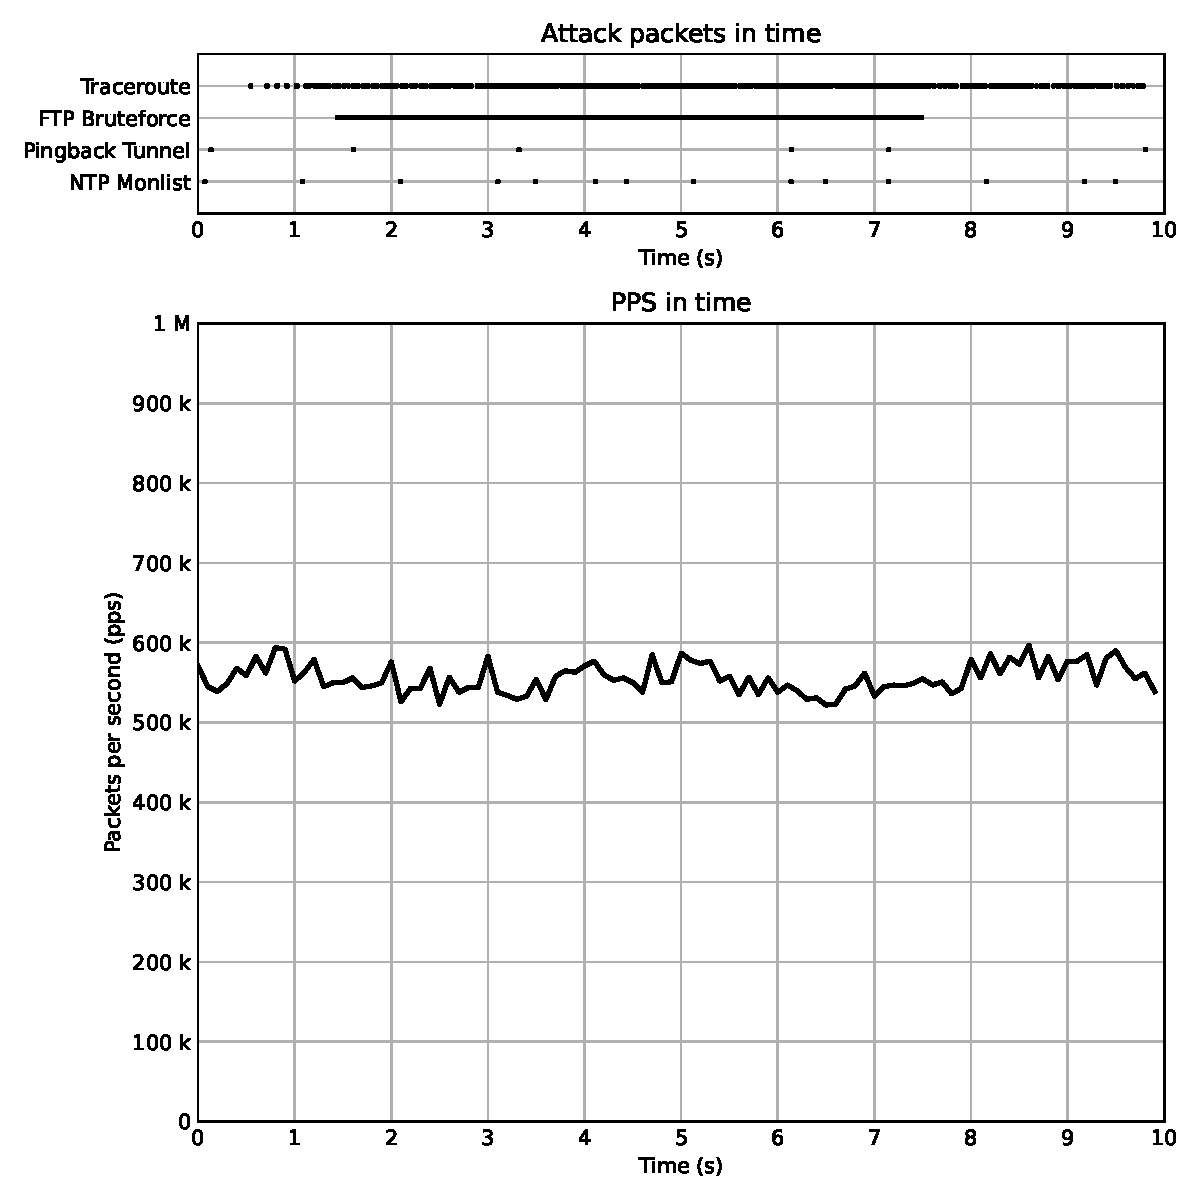
\includegraphics[width=0.7\textwidth]{images/pps_in_time.pdf}  
    \end{center}
    \label{fig:pps_in_time}
    \legend{Source: the author (2022).}
\end{figure}

% Explain the dataset (with plots) + attacks + ferramentas para gerar dataset
% - datasets status: taxa de pico, pps, total size, duration, packets, characteristics...
% - Attacks:
% - FTP Bruteforcing
% - Pingback https://github.com/corelight/pingback
% - Detect traceroute
% - NTP Monlist



\subsection{Experiment setup and methodology}
\label{sec:evaluation:setup}

In this section, we describe the setup of our experiment. The experiment used the same technologies described in \autoref{sec:evaluation:deployment}, relying on network virtualization, P4 emulation to run our switch, and containerization to run Zeek. The objective of our evaluation was to compare the functionality and performance of the Zeek Scripts without RNA compared with RNA.

Switch emulation does not perform as fast as a real P4 hardware switch, which makes it impossible for us to execute our experiment with a P4 switch in real-time since we only use emulated switches. In this scenario, the emulated switch would become a bottleneck, preventing the traffic from reaching Zeek at the same rate as it enters the P4 pipeline. For this reason, we assess only the performance of the Zeek monitoring system. We assume that a (hardware) programmable forwarding device would be able to execute the program at line rate if the provided program fits the device's memory.

\vspace{1em}

To overcome the performance deficit of emulated P4 switches, we process the combined dataset before running the experiment, effectively creating a second dataset. This second dataset represents a real-world output of a P4-switch, receiving our combined dataset and processing it at line rate. We call this second dataset the \textit{RNA dataset}.

To explain the generation of this second dataset, we use \autoref{fig:rna_dataset_diagram}. The first step is to select from our dataset only the packets that may trigger an Offloader, which will eventually generate an mRNA message. With this intermediate trace, we execute our emulated P4 switch, which is now able to process the dataset faster due to the decreased amount of traffic. This results in a dataset with only mRNA messages, the \textit{RNA dataset}. It is also important to note that in all datasets during this process, all packets have their timestamps preserved, and real behavior is emulated.

\begin{figure}[htb]
    \caption{RNA dataset creation diagram}
    \begin{center}
        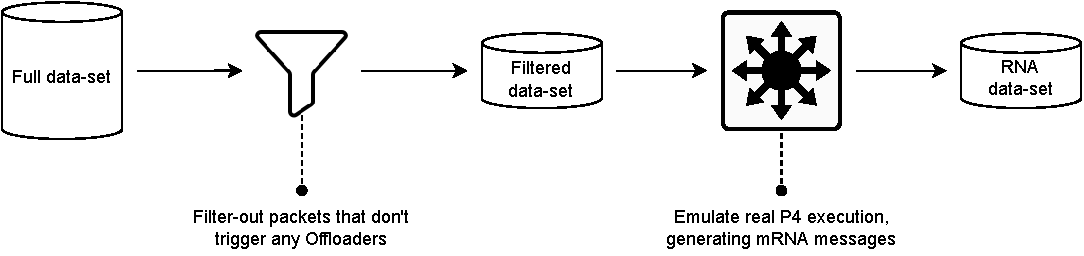
\includegraphics[width=1.0\textwidth]{images/rna_dataset_creation.pdf}  
    \end{center}
    \label{fig:rna_dataset_diagram}
    \legend{Source: the author (2022).}
\end{figure}

Now that we have our two datasets, the \textit{combined dataset} and the \textit{RNA dataset}, we need to execute Zeek in both scenarios and compare its output and performance. This is done by running Zeek in a Docker container connected to the host computer by a virtual network interface. In this network interface, we replay those two traces, one at a time, and record the memory and CPU usage. Each scenario was executed fifteen times to account for variability. The experiments were executed on a notebook with an Intel Core i9-10885H (\SI{5.3}{GHz}, 8 cores, 16 threads) CPU, \SI{16}{GB} ($2 \times$\SI{8}{GB}) of DDR4 RAM (\SI{3200}{MT/s}), and a \SI{1}{TB} NVMe SSD. While the experiments were executed, in order not to affect the results, no other non-essential services were executed on the computer.

% Methodology?

% \subsection{Methodology}

% Explain results
% - accuracy
%   + script count
% - development cost savings (and less prone to development mistakes)
%   - Show table with multiple combinations of scripts: [1], [2], [3], [4], [1, 2, 3, 4]
% - performance gain
%   - memory, cpu, (execution time/detection time)


\subsection{Results}

In this section, we describe the results of the experiment and functional assessment of our code generation mechanism. We first present the functional results, answering research questions one (RQ1) and two (RQ2). We later present the performance results, answering \textit{RQ3}.

\subsubsection*{Functional results}

To assess whether our proposed mechanism works, we used our prototype and the attacks dataset to compare the output of a Zeek deployment with and without RNA. After executing both setups and comparing the output of Zeek's \textit{notices}, we concluded that our code generation mechanism was able to generate code to successfully offload four different scripts, namely \textit{FTP Bruteforcing}, \textit{Detect traceroute}, \textit{ICMP Pingback}, and \textit{NTP Monlist}. All of these scripts were able to detect, with complete accuracy, all the attacks present in the workload of the experiment, resulting in no difference between the execution with and without RNA in terms of detection.

To answer the second question, we manually inspect the generated code for RNA. Our objective is to check whether our approach is helpful and facilitates the deployment of RNA. \autoref{tab:lines_per_script_count} summarizes the main results obtained. The generated output instance of RNA for offloading our four Zeek Scripts (described above in this section) has $2967$ lines of code. To develop a new Protocol Template, according to \autoref{tab:lines_by_protocol_template}, a median of $40$ lines of code would need to be written, and for a new Offloader Template (\autoref{tab:lines_by_offloader_template}), a median of $224$. This gives developers a big advantage over writing a fully standalone solution since templates are small and easier to maintain than a complete solution. The main advantage leans on the reuse of Protocol and Offloader Templates. Using templates, a network operator is able to deploy RNA without writing a single line of code, only with a command. The automatic code generator identifies the needed events to offload the desired scripts and generates the complete code.


\begin{table}[htb]
    \caption{Lines of Code per Script Count}
    \begin{center}
        \begin{tabular}{|l|r|}
            \hline
            \textbf{Monitoring Script Count} & \multicolumn{1}{l|}{\textbf{Generated Lines Median}} \\ \hline
            1 Monitoring Script              & 2113.5                                             \\ \hline
            2 Monitoring Scripts             & 2421.5                                             \\ \hline
            3 Monitoring Scripts             & 2714.0                                             \\ \hline
            4 Monitoring Scripts             & 2967.0                                             \\ \hline
        \end{tabular}%
    \end{center}
    \label{tab:lines_per_script_count}
    \legend{Source: the author (2022).}
\end{table}

\begin{table}[htb]
    \caption{Lines of code of Protocol Templates}
    \begin{center}
        \begin{tabular}{|l|r|r|r|}
            \hline
            \textbf{Protocol Template} & \multicolumn{1}{l|}{\textbf{Lines of Configuration}} & \multicolumn{1}{l|}{\textbf{Lines of code}} & \multicolumn{1}{l|}{\textbf{Total Lines}} \\ \hline
            Ethernet Protocol          & 13                                                   & 13                                          & 26                                        \\ \hline
            IPv4 Protocol              & 17                                                   & 26                                          & 43                                        \\ \hline
            IPv6 Protocol              & 17                                                   & 20                                          & 37                                        \\ \hline
            ICMP Protocol\footnotemark & 59                                                   & 77                                          & 136                                       \\ \hline
            TCP Protocol               & 22                                                   & 45                                          & 67                                        \\ \hline
            UDP Protocol               & 21                                                   & 10                                          & 31                                        \\ \hline
            \textit{Total}             & \textit{149}                                         & \textit{191}                                & \textit{340}                              \\ \hline
            \textit{Median}            & \textit{19}                                          & \textit{23}                                 & \textit{40}                               \\ \hline
        \end{tabular}%
    \end{center}
    \footnotetext{TODO}
    \label{tab:lines_by_protocol_template}
    \legend{Source: the author (2022).}
\end{table}

\begin{table}[htb]
    \caption{Lines of code of Offloader Templates}
    \begin{center}
        \begin{tabular}{|l|r|r|r|}
            \hline
            \textbf{Offloader Template}        & \multicolumn{1}{l|}{\textbf{Lines of Configuration}} & \multicolumn{1}{l|}{\textbf{Lines of code}} & \multicolumn{1}{l|}{\textbf{Total Lines}} \\ \hline
            NTP Message                        & 27                                                   & 152                                         & 179                                       \\ \hline
            ICMP Echo Message                  & 28                                                   & 157                                         & 185                                       \\ \hline
            ICMP Time Exceeded & 28                                                   & 305                                         & 333                                       \\ \hline
            FTP Request and Reply              & 28                                                   & 235                                         & 263                                       \\ \hline
            \textit{Total}                     & \textit{111}                                         & \textit{849}                                & \textit{960}                              \\ \hline
            \textit{Median}                    & \textit{28}                                          & \textit{196}                                & \textit{224}                              \\ \hline
        \end{tabular}%
    \end{center}
    \label{tab:lines_by_offloader_template}
    \legend{Source: the author (2022).}
\end{table}


% \begin{figure}[htb]
%     \caption{Generated lines per script count}
%     \begin{center}
%         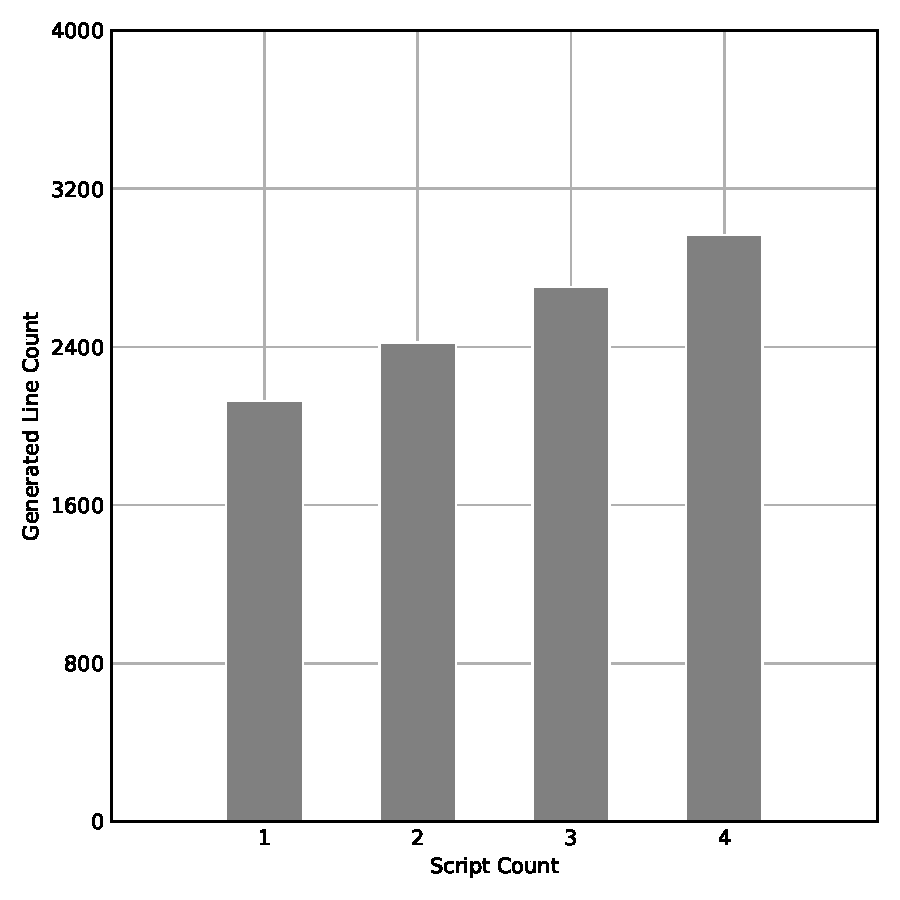
\includegraphics[width=0.7\textwidth]{images/generated_lines.pdf}  
%     \end{center}
%     \label{fig:gen_lines_per_script}
%     \legend{Source: the author (2022).}
% \end{figure}


\subsubsection*{Performance results}

To answer our third research question and assess the performance gain of offloading scripts with RNA, we replayed both of our datasets, the \textit{combined dataset}, and the \textit{RNA dataset}. When replaying the RNA dataset, we enabled our Zeek Plugin, which processed the incoming mRNA messages. This resulted in a significant gain in performance. As Figure \ref{fig:rna_perf} shows, the mean CPU\footnote{Usage of one CPU core. $100\%$ represents usage of a full core, $150\%$ represents usage of one and a half CPU cores.} usage without RNA is $109\%$, and memory usage reaches a maximum of $960.64$ MB by the end of the experiment. With RNA (simulated by using the \textit{RNA dataset}), mean CPU utilization was $1.9\%$ and the maximum memory usage was $235.07$ MB. Additionally, without RNA, a mean of $35.24\%$ of the packets was dropped. The high dropped packet rate resulted in one of the attacks, the \textit{FTP Bruteforce Attack}, not being detected in $93.3\%$ of the iterations executed without RNA. Using our approach, no packets were dropped, and all attacks were detected in all executions of the experiment.

In \autoref{fig:rna_perf}, at time \SI{5}{s}, we observe a significant change in the increase of memory and CPU usage. Our hypothesis is that this is the moment internal Zeek buffers are filled, decreasing the rate packets are read, slowing down the increase of memory usage, and increasing the CPU usage. In a real-world scenario, network operators would not allow an IDS to drop packets and would increase the processing power or implement a sampling strategy. Our intention with this comparison is to contrast the usage of a normal Zeek deployment compared to our RNA framework, which uses Programmable Data Planes to offload IDS operations. Nevertheless, our results suggest that the observed reduction in CPU usage for the RNA-based setup would allow for the use of a smaller cluster for the given scenario. 

Another important note is that the Dynamic Protocol Detection (DPD), which we presented in \autoref{sec:bg:zeek_ee}, is unable to dynamically detect protocols when RNA is used, potentially resulting in better performance, giving RNA an advantage. This is also one of the assumptions we made to simplify the development of the mechanism.

% Metrics:
% 1. How many scripts we can run (without intervention)
% 2. How many lines were produced per script
%     a. Include copied from the template (maybe create a table with the outline)
% 3. Performance gain in offloading (optional): compare a raw data set vs mRNA messages data set.
%     a. memory, cpu, execution time

\begin{figure}[htb]
    \caption{RNA Performance Evaluation}
    \begin{subfigure}{.5\textwidth}
        \centering
        \vspace{1em}
        \caption{CPU usage by time}
        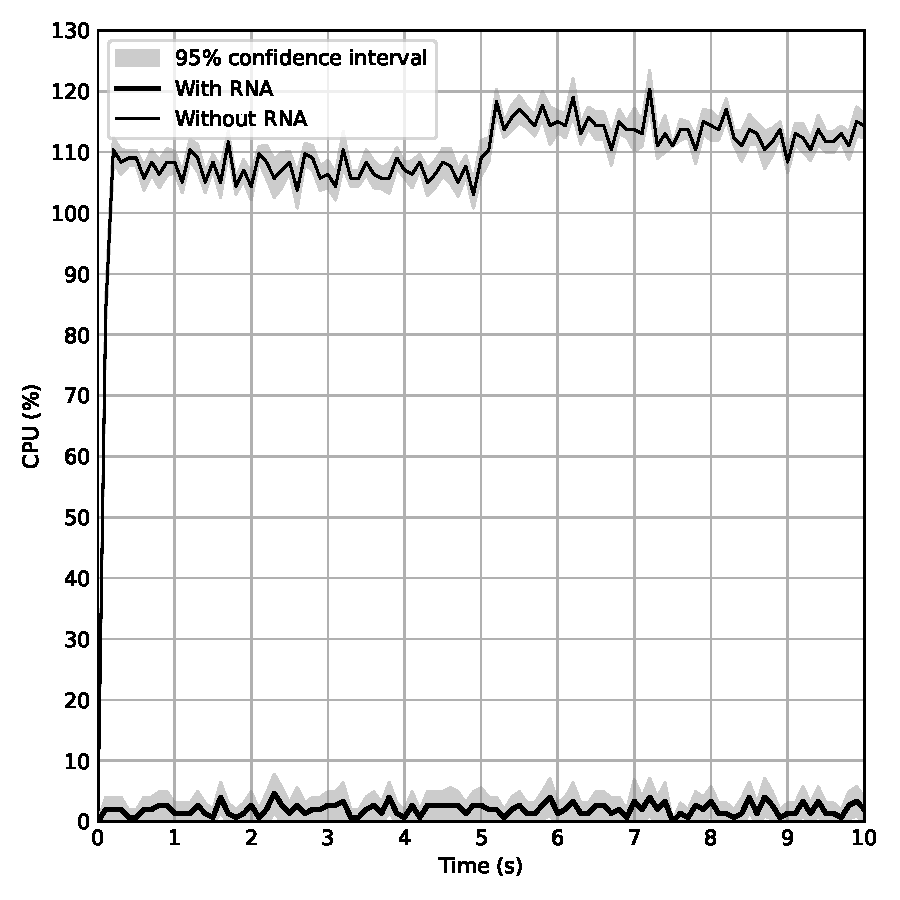
\includegraphics[width=1.0\textwidth]{images/aggregated_cpu_plot.pdf}
        \label{fig:rna_cpu}
    \end{subfigure}%
    \begin{subfigure}{.5\textwidth}
        \centering
        \vspace{1em}
        \caption{Memory usage by time}
        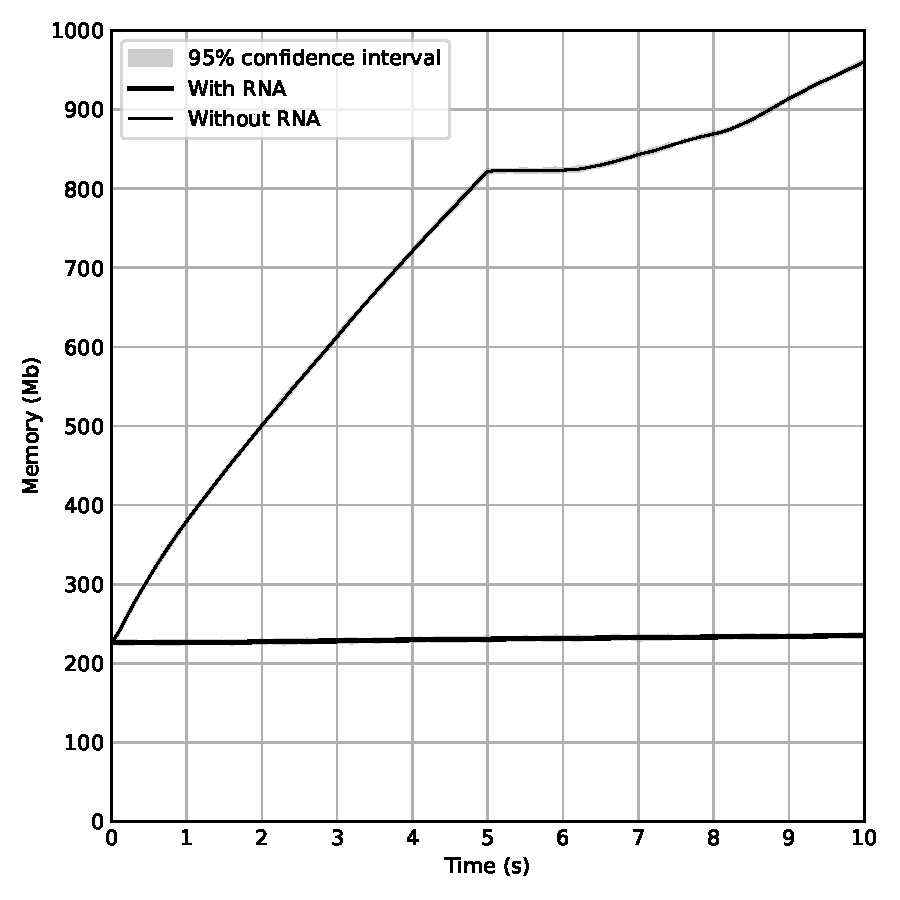
\includegraphics[width=1.0\textwidth]{images/aggregated_memory_plot.pdf}
        \label{fig:rna_mem}
    \end{subfigure}
    \label{fig:rna_perf}
    \legend{Source: the author (2022).}
\end{figure}

% 
% ====================       Pode revisar até aqui :)       ====================
% 
      % 5
\chapter{Conclusion}
\label{cap:conclusion}

In this project, we investigated the benefits of using Programmable Data Planes to offload Zeek monitoring scripts. We also took the first step towards an automatic code generation mechanism, which enables any network operator without programming knowledge to offload Zeek scripts to programmable forwarding devices. We implemented an automatic code generator that identifies which Zeek Events are required by a set of scripts and, using templates, automatically generates P4 and Zeek code to offload these scripts.

After proposing additions to the RNA framework and implementing our prototypical automatic code generator, we evaluated the proposed approach and assessed its capabilities of automatically generating code and enhancing performance. We showed the mechanism generates almost $3$ thousand lines of code, which, otherwise, a developer would need to write manually in order to offload four Zeek Scripts. We demonstrated that RNA can give a performance benefit compared to server-based intrusion detection, resulting in $57\times$ less CPU usage and $4\times$ less memory usage for the workload used in the experiments. Moreover, we have also shown that our approach can produce these benefits for network operators without any previous P4 programming knowledge. It is also important to note that these results are still to be confirmed with future experiments using hardware PFDs.

%\vspace{-0.5em}

%\section{Challenges and Difficulties}

%\vspace{-0.5em}
% "Reflexão pessoal", desafios do projeto (1 parágrafo)

%This project's main challenge was adapting an existing IDS, in our case Zeek, to work with PDP offloading. This adaptation was also challenging due to the lack of internal documentation on the Zeek internal subsystems, initially designed to facilitate adding support to new protocols without needing to modify the existing data flow.

% \section{Future Work}

This project took the first step towards adding automatic code generation to RNA. Next, we describe some opportunities for future work and items that could be improved. These items are both suggestions for RNA and the code generator mechanism.

\subsubsection*{Stateful Connections}

The next step to allow better protocol handling, mainly of TCP connections, is the implementation of stateful analysis into RNA. Stateful analysis will allow far more significant performance benefits if executed in the data plane. It will offload a significant part of Zeek state management, allowing P4 to analyze more connection-based protocols.


\subsubsection*{Multiple Offloaders}

At the current state of RNA and our code generation mechanism, it is not possible to trigger more than one Offloader per incoming packet. This limitation could impact future deployments where many scripts are being executed. This is a problem that should be solved in the future.


\subsubsection*{Enhanced Zeek \textit{Connection} Management}

Zeek uses an object called \textit{Connection} (not to be confused with an actual \textit{network connection}) to manage sessions internally. This object is not deallocated after usage in our aproach. Future work must develop a mechanism to handle protocol timeouts and free resources after these are no longer needed. Some protocols also have timeout events, which should also be triggered by the PDP.

      % 1

% Bibliograpy

\bibliographystyle{abntex2-alf}
\bibliography{biblio}

% Appendixes
\appendix

\chapter{Example of a Protocol Template}
\label{cap:protocol_template}

\begin{figure}[htb]
    \centering
    \caption{Template configuration file: \texttt{icmp.hjson}}
    \lstinputlisting[style=hjson]{code/icmp_template/icmp.hjson.txt}
    \label{code:icmp_template:config}
    %\vspace{-1em}
\end{figure}

\begin{figure}[htb]
    \centering
    \caption{Template header file: \texttt{icmp\_header.p4.txt}}
    \lstinputlisting[style=p4]{code/icmp_template/icmp\_header.p4.txt}
    \label{code:icmp_template:header}
\end{figure}

\begin{figure}[htb]
    \centering
    \caption{Template ingress processor file: \texttt{ingress\_processor.p4}}
    \lstinputlisting[style=p4]{code/icmp_template/ingress\_processor.p4.txt}
    \label{code:icmp_template:ingress_processor}
    %\vspace{-1em}
\end{figure}
\chapter{Example of an Offloader Template}
\label{cap:offloader_template}

\end{document}
